\chapter{MEC Neurons Encode Subsets of Navigational Variables}
\label{chapterlabel5}
After the discovery of grid cells in MEC, an explosion of literature on MEC cell characterisation shows that rat MEC contains grid cells, speed cells, head direction cells, boundary vecotr cells, conjugative cells, etc. In addition, rat MEC cells can have multiplexed and heterogeneous codes and this finding applies a multivariate generalised linear model to find tunings for speed, 2D space, head direction, theta phase together. However, mice are found to have 0-10\% grid cell yield and the representation can drift over time. Further to that, most mice MEC research focused on VR studies to make advantage of this tool with high yield recording devices. This approach, including this thesis, restrains the spatial tuning to be one-dimensional and focuses on partial functions of MEC. For example, focuses on cue-tuning, focuses on distance-tuning, tried to identify grid cells with spatial spectrogram and how they evolve in more visually-dominated environments. These selective approaches provide many insights on MEC's role in mutiple contexts and how diverse MEC can be. However, there still lacks a comprehensive characterisation of MEC cells' roles together in VR setting. In this chapter, by the advantage of using visually-complex environments in this thesis, a similar multiplexed and heterogeneous population code is found in mouse MEC with some deviations from previous findings. 

\section{Method}
\subsection{Spatial Tuning}
Cells with 95\% peak percentile from shuffled data in the two tracks, > 0.1Hz mean firing rate in the tracks and median variance > 0.6 across 10 folds of all laps (removes neurons only fire in some random laps). Spikes are first smoothed with 200 ms gaussian window in time at 60 Hz and binned at 2 cm bins. The spatial bins are extended to final position where the gray screen ends (3-5s after the lap finishes at 140 cm) to trace the post-VR dynamics.

\subsection{Speed Tuning}
Speed response is binned at 1 cm/s bin from 0 cm/s to 40 cm/s. A skewed gaussian line fitting is applied to binned speed response from (citation):
equation

The skewed peak is defined as which speed the neuron prefers, which is divided into untuned (\(R^2 < 0.15\)), low-pass, band-pass (5, 10, 15, 20, 25, 30), and high-pass.



\section{Results}
\subsection{MEC Population Remaps in the Two Tracks}
The population codes in MEC remap in the two tracks across sessions. In Fig 5.1A, there are three population maps of the MEC neuronal activities. On the left is the normalised average of track 1 responses in even laps and sorted by the peaks of track 1 normalised average responses in odd laps and the map is extended to 200cm (60cm longer than the VR during gray screen between laps). In the middle panel is the track 2 normalised average responses from even laps and it is sorted by peaks in track 1 odd laps. On the right hand is the track 2 normalised average responses in even laps sorted by peaks in track 2 normalised average responses in track 2 odd laps. This tests if track 2 has similar population response as track 1 when it is sorted by track 1 odd laps, and the track 1 odd laps sorting particularly does not work for middle part of VR. For the start of the VR positions and end of VR/ reward locations, many neurons do not remap. In addition, many neurons have sharp peak or suppression around 130 cm in track 1 and 145 cm in track 2, and many neurons have more peaks in track 2. To further test if many neurons remap in the two tracks, Pearson correlation is calculated between four pairs: T1 even |T1 odd vs T1 odd | T1 odd ( within track 1), T2 even | T2 odd vs T2 odd | T2 odd (within track 2), T2 even | T2 odd vs T1 even | T2 odd (across tracks), T2 odd | T2 even vs T1 odd | T2 even (across tracks). The acros- track pairs have correlations centre around 0.2 ranging from -0.4 to 0.9 whereas within-track pairs have correlations centre around 0.4 ranging from -0.2 to 1 (Fig 5.1B).

\subsection{Diverse Spatial Tuning Profiles}
MEC neurons have diverse spatial tuning profiles with remapping, partial remapping and no remapping. In Fig 5.1C, 5 example neurons with high stability are shown and the shapes on top are labelled in Fig 5.1A. In first neuron, it is tuned to centre of the VR with 4 peask in T1 and only 2 peask in T2 but highly overlapping with T1's two peaks. In second neuron, the tuning is highly similar in the two tracks except for the peaks at 140 cm in T1 and 155 cm in T2, and these two different peaks differ by 15 cm which is the difference in reward zone positions in the two tracks. This difference is also shown on the 5th example neuron which shows a suppression instead of peaks and this effect is particularly obvious in the population map in Fig 5.1A. Both 3rd and 4th example neurons (Fig 5.2C) have more peaks in track 2 than track 1 and there are many neurons with these extra peaks in track 2 (FIg 5.1A). In addition, the 3rd example neuron has an almost identical peak at the start of the VR in both tracks (Fig 5.1C).
\begin{figure}
    \centering
    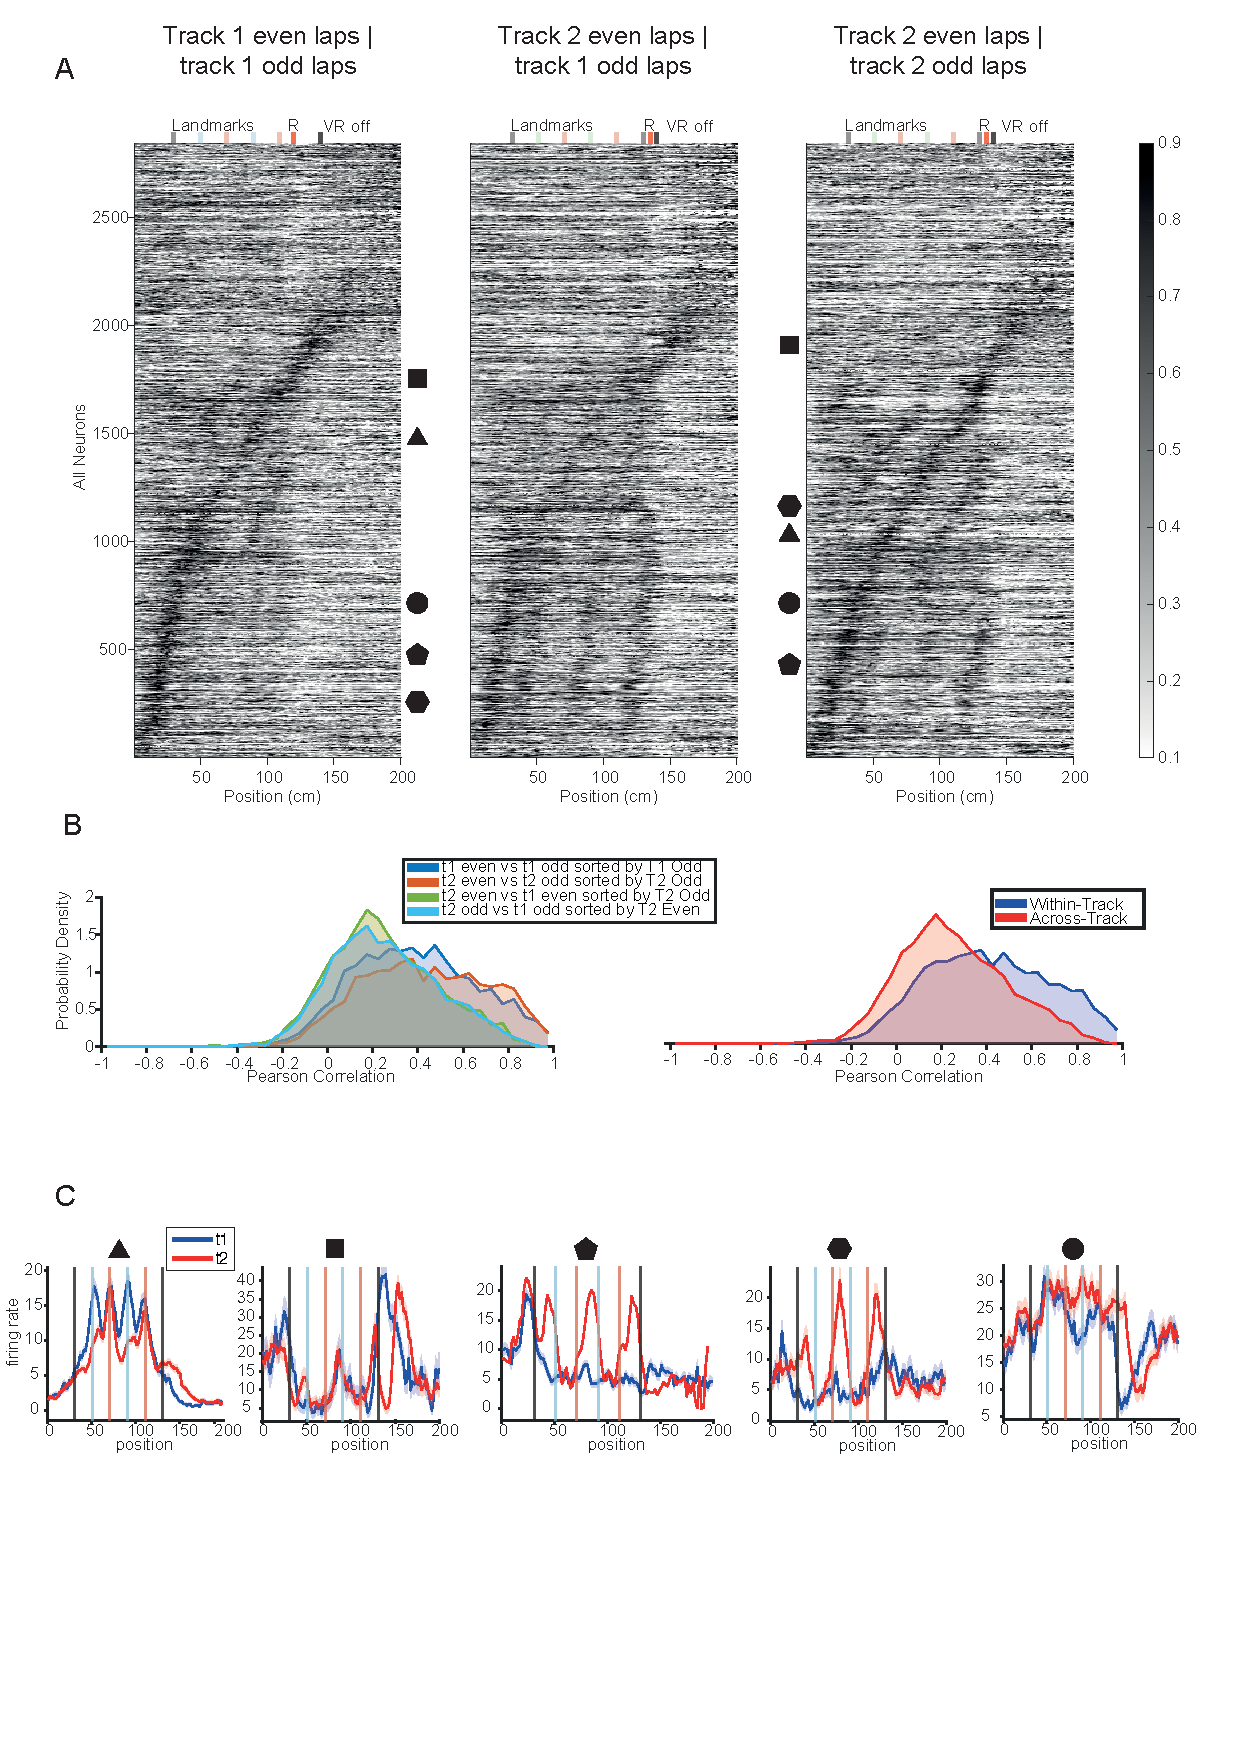
\includegraphics[width=1\linewidth]{figures//Chapter 5 MEC/fig1_MEC_spatial_tuning.pdf}
    \caption{MEC neurons are spatially tuned to positions in two environments and remap in the two environments.}
    \label{fig:MEC remapping}
\medskip
\small
\textbf{A)} Population maps of all MEC cells across sessions. From left to right is normalised average responses from either Track 1 or Track 2 even laps sorted by either peak locations in Track 1 odd laps or Track 2 odd laps. The position bin is extended outside of the VR during gray screen period between laps and the landmarks, rewards and VR off positions are labeled aobve the maps. \textbf{B)} Pearson correlation between two population maps in four pairs. Both panels are the same comparison but the one on the right merges pairs within track and pairs across track together. \textbf{C)} 5 example MEC neurons with high stability which show different degrees of spatial tuning and remapping. They are also labeled on panel \textbf{(A)}.
\end{figure}

\subsection{Speed Tuning}
In addition to spatial tuning, many MEC cells are tuned to the animal's running speed and some neurons have different speed tuning than linearly increasing speed cells in previous literature. The firing rate of the cell is binned by the animal's running speed and plotted in log scale in Fig 5.2A. A skewed gaussian curve is fitted to the responses. The peak of the best fit gaussian curve is what the cell is tuned to which is the preferred speed. The preferred speed is categorised into low-pass ( < 5 cm/s) , band-pass (5-30 cm/s), and high-pass ( > 30 cm/s). Many neurons have good fitting with this gaussian curve (Fig 5.2A) and there are cells tuned to all types of classifications: about 30\% not tuned, about 10\% low pass, about 5\% for each band of 5-20 band-pass, about 30\% for above 25 cm/s speeds. The gaussian curve fitting accounts for the linear increase in high speed preference cells which are likely speed cells found in previous literature. Beyond the classified cells, there are some cells classified as not tuned, for example the bottom right two example neurons in Fig 5.2 A, show more complex speed tuning where the middle one looks like an oscillation and the right-most one has high firing rate when stationary and firing rate increased after 20 cm/s speed. The gaussian curve fitting method works very well for many cells but can miss cells with complex tuning curve.
\begin{figure}
    \centering
    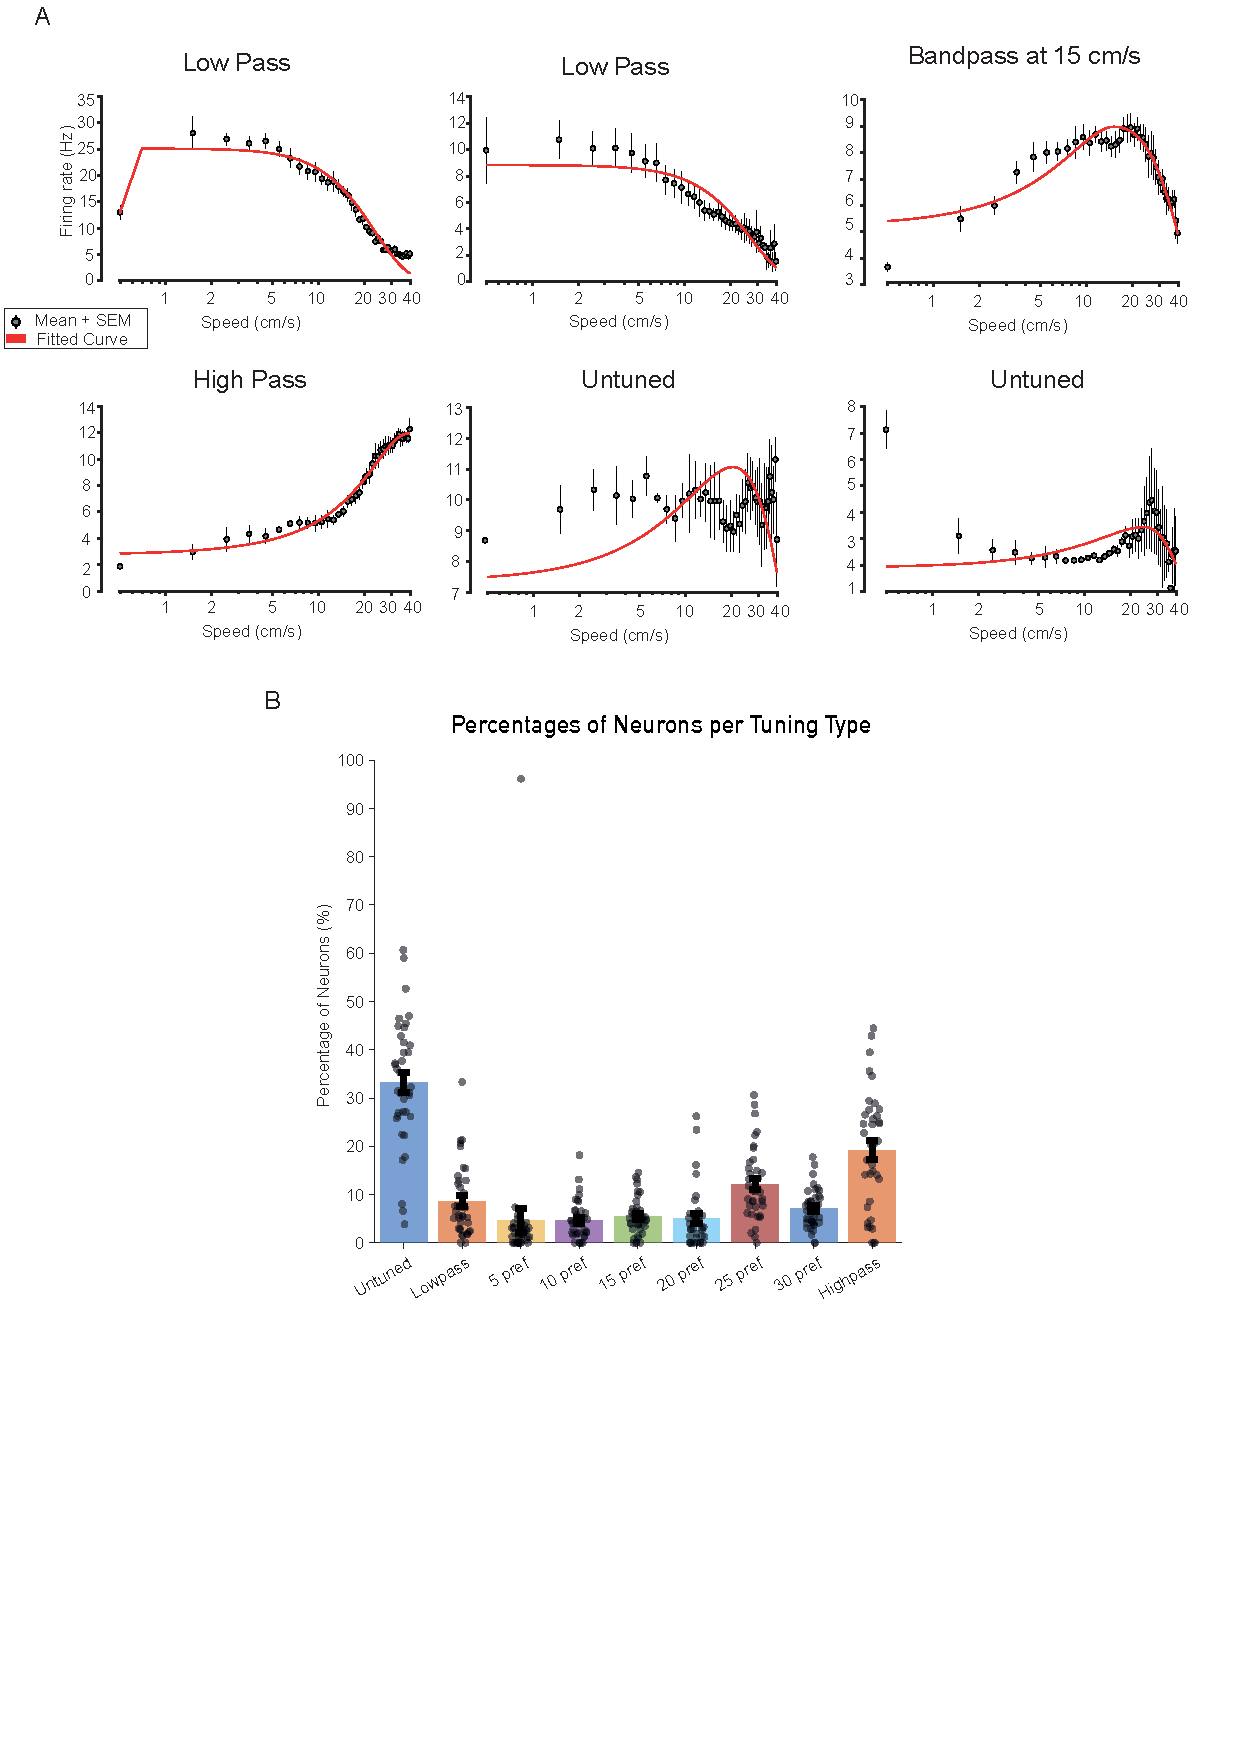
\includegraphics[width=1\linewidth]{figures//Chapter 5 MEC/fig2_speed_tuning.pdf}
    \caption{Speed Tuning in MEC}
    \label{fig:placeholder}
\medskip
\small
\textbf{A)} 6 example neurons' speed tuning. The x coordinate of animal's speed is in log scale. Each dot and its error bar is the neuron's firing rate at that speed. A fitted skewed gaussian curve in red is fitted to find the preferred speed of the neuron. \textbf{B)} Total percentages of neurons tuned to different speeds across sessions.
\end{figure}

\subsection{Multi-variate Tuning in MEC Cells}
MEC cells have subpopulations tuned to multiple variables and the interaction between variables can be additive or multiplicative at neuronal level. As described in previous V1 neuron characterisation chapter, a \(Speed \times Position \) binning method was used to compare speed impact on spatial binning. Here, the same method is used to understand the relationship between speed tuning and spatial tuning. In Fig 5.3A and Fig 5.3F, two example neurons with low-pass speed tuning and high-pass speed tuning respectively. In Fig 5.3A, the neuron has the low-pass speed tuning effect on the first spatial peak at the start of VR but the peaks at the end of VR around 135-160 cm have high firing rate at the peak positions whatever the animal's running speed is. In Fig 5.3F, the neuron has high-pass speed tuning effect on all the positional tuning across the VR from 30-150 cm in both tracks, but the neuron has no speed tuning at all in the rest including start of the VR and the gray screen period. In addition, the difference in position of the last peaks in track 1 and track 2 in Fig 5.3A and Fig 5.3B and the extra peak in track 2 of Fig 5.3F and Fig 5.3G can potentially be contributed by the reward responses as the reward zone is 115-125 cm in track 1 and 130-140 cm in track 2. In order to understand the multi-variate tuning in MEC cells, a generalised linear model is applied to the cells. The model has 5 cm bin spatial predictors for each track and speed predictors at 2.5 cm/s bins and a reward predictor at [0, 0.5]s time range. A ridge regression is applied to the GLM with a normal distribution. 
\begin{figure}
    \centering
    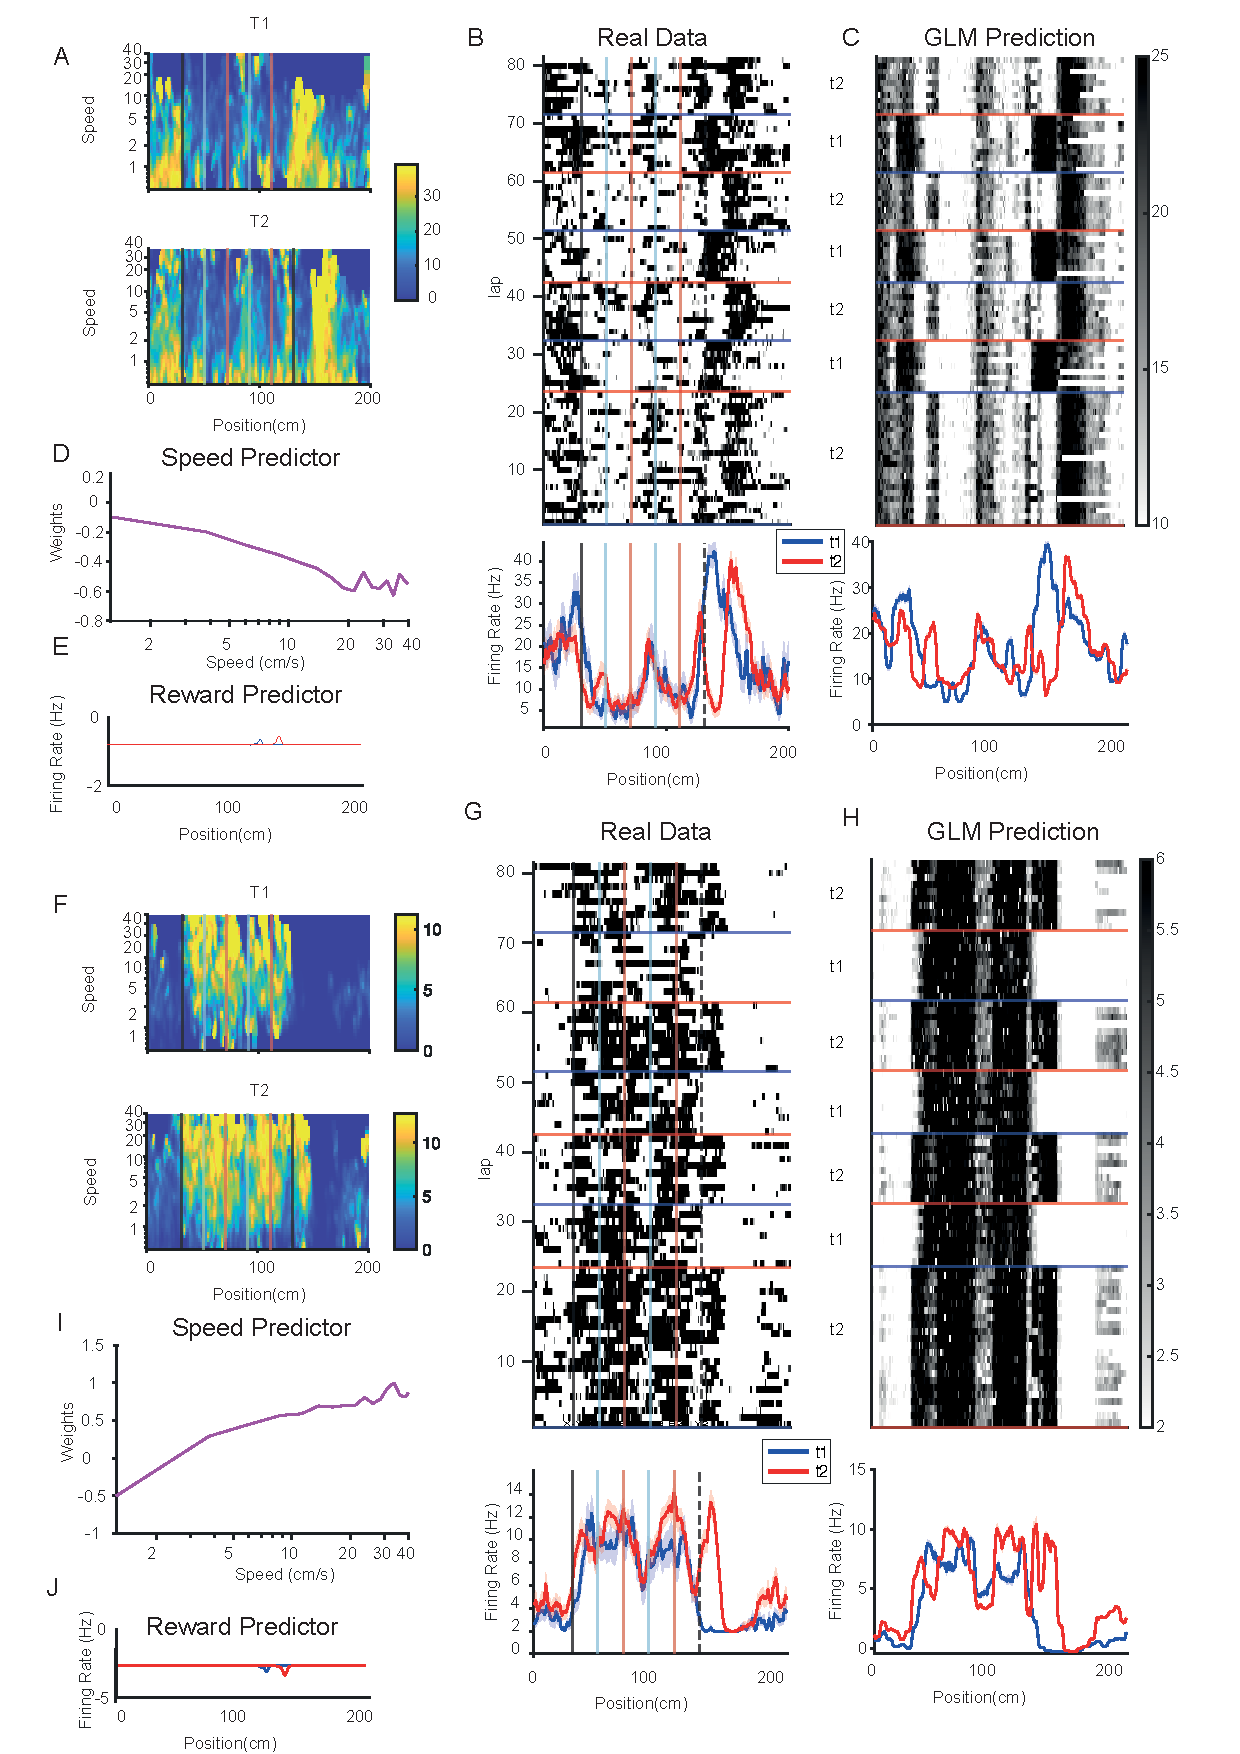
\includegraphics[width=1\linewidth]{figures//Chapter 5 MEC/fig3_multiple_navigational_variables.pdf}
    \caption{MEC Cells Tuned to Multiple Navigational Variables}
    
    \label{fig:placeholder}
\medskip
\small
In this figure, two example neurons are displayed and they separated by top and bottom rows. \textbf{A,F)} Firing rate is binned by \(Speed \times Position\) to show the impact of speed tuning on spatial tuning and top panel is track 1 and bottom panel is ttrack 2. \textbf{B, G)} The raster plots across the tracks of two example neurons and their PSTHs in the two tracks. \textbf{C, H)} Same as \textbf{(B,G)} but using predicted firing rates from a trained GLM model. \textbf{D, I)} Speed predictors' weights from the GLM model. \textbf{E, J)} Reward predictors' impact in the two tracks on the PSTH.
\end{figure}



\begin{figure}
    \centering
    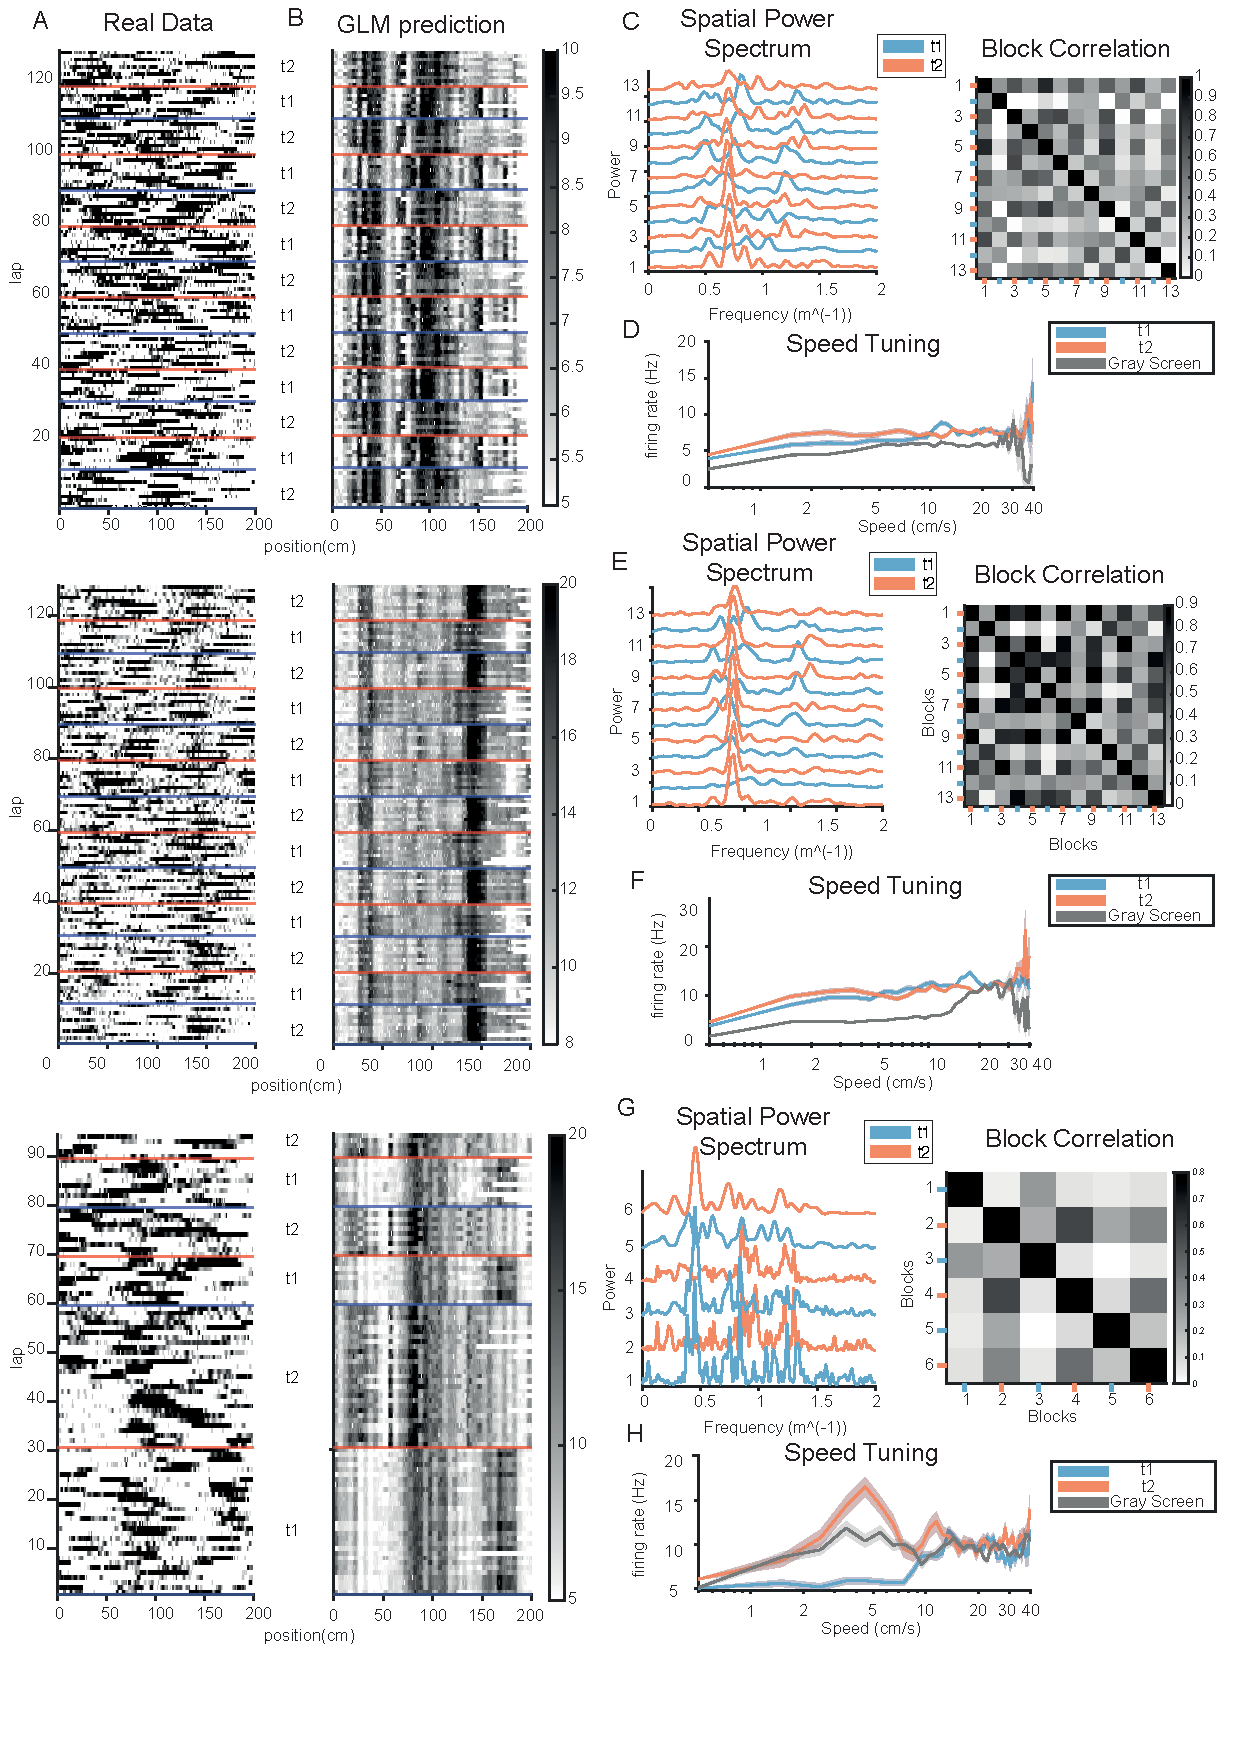
\includegraphics[width=1\linewidth]{figures//Chapter 5 MEC/fig4_periodic_firing.pdf}
    \caption{Periodic Firing Cells in MEC}
    \label{fig:placeholder}
    \medskip
\small
In this figure, two example neurons are displayed and they separated by top and bottom rows. \textbf{A,F)} Firing rate is binned by \(Speed \times Position\) to show the impact of speed tuning on spatial tuning and top panel is track 1 and bottom panel is ttrack 2. \textbf{B, G)} The raster plots across the tracks of two example neurons and their PSTHs in the two tracks. \textbf{C, H)} Same as \textbf{(B,G)} but using predicted firing rates from a trained GLM model. \textbf{D, I)} Speed predictors' weights from the GLM model. \textbf{E, J)} Reward predictors' impact in the two tracks on the PSTH.
\end{figure}
\subsection{MEC Has a Subpopulation with Periodic Firing}
